%%% Local Variables: 
%%% mode: latex
%%% TeX-master: t
%%% End: 

\chapter{从局部到全局的配准策略}
\label{cha4}

\section{局部初始配准}
\subsection{环-血管特征}
在上章中,我们提到:为保证配准的准确性,我们只采用参考图像和待配准图像中最优的三点环、四点环和五点环作为配准环结构,同时对它们进行多环的组合以最大限度提高配准结果的准确率。然而,上述措施对于配准来说仍然是不充分的:一方面,这使得一些图片只包含有限的环特征点,而后续的图像空间坐标变换需要足够的匹配的特征点来得到变换参数,另一方面,环结构只占据整个视网膜图像中较小的一部分,我们实际使用的只是视网膜血管的分叉点或交叉点,而没有考虑到视网膜的血管信息。血管是视网膜图像中占据面积最大,也是较稳定的特征之一,而在环结构周围的血管同时也具有唯一性,因此将血管上的点也加入到特征点中具有可行性。

综上,我们提出了环-血管特征用来完成视网膜图像的局部初始配准,环-血管特征由环结构,与环结构上的每个特征点沿血管最近的分叉点、交叉点或结束点(可能是血管末梢或血管上的一段)两者之间的血管的中点组成。环-血管特征不仅增加了特征点的数量,扩大了环结构在图像上的占有范围,还加入了血管的信息,因而更有利于后续准确地求解坐标变换参数及配准工作。如图~\ref{5bifur-vess}所示,蓝色为五点环,粉红色为其血管点。
   \begin{figure}[ht!]
   \centering
  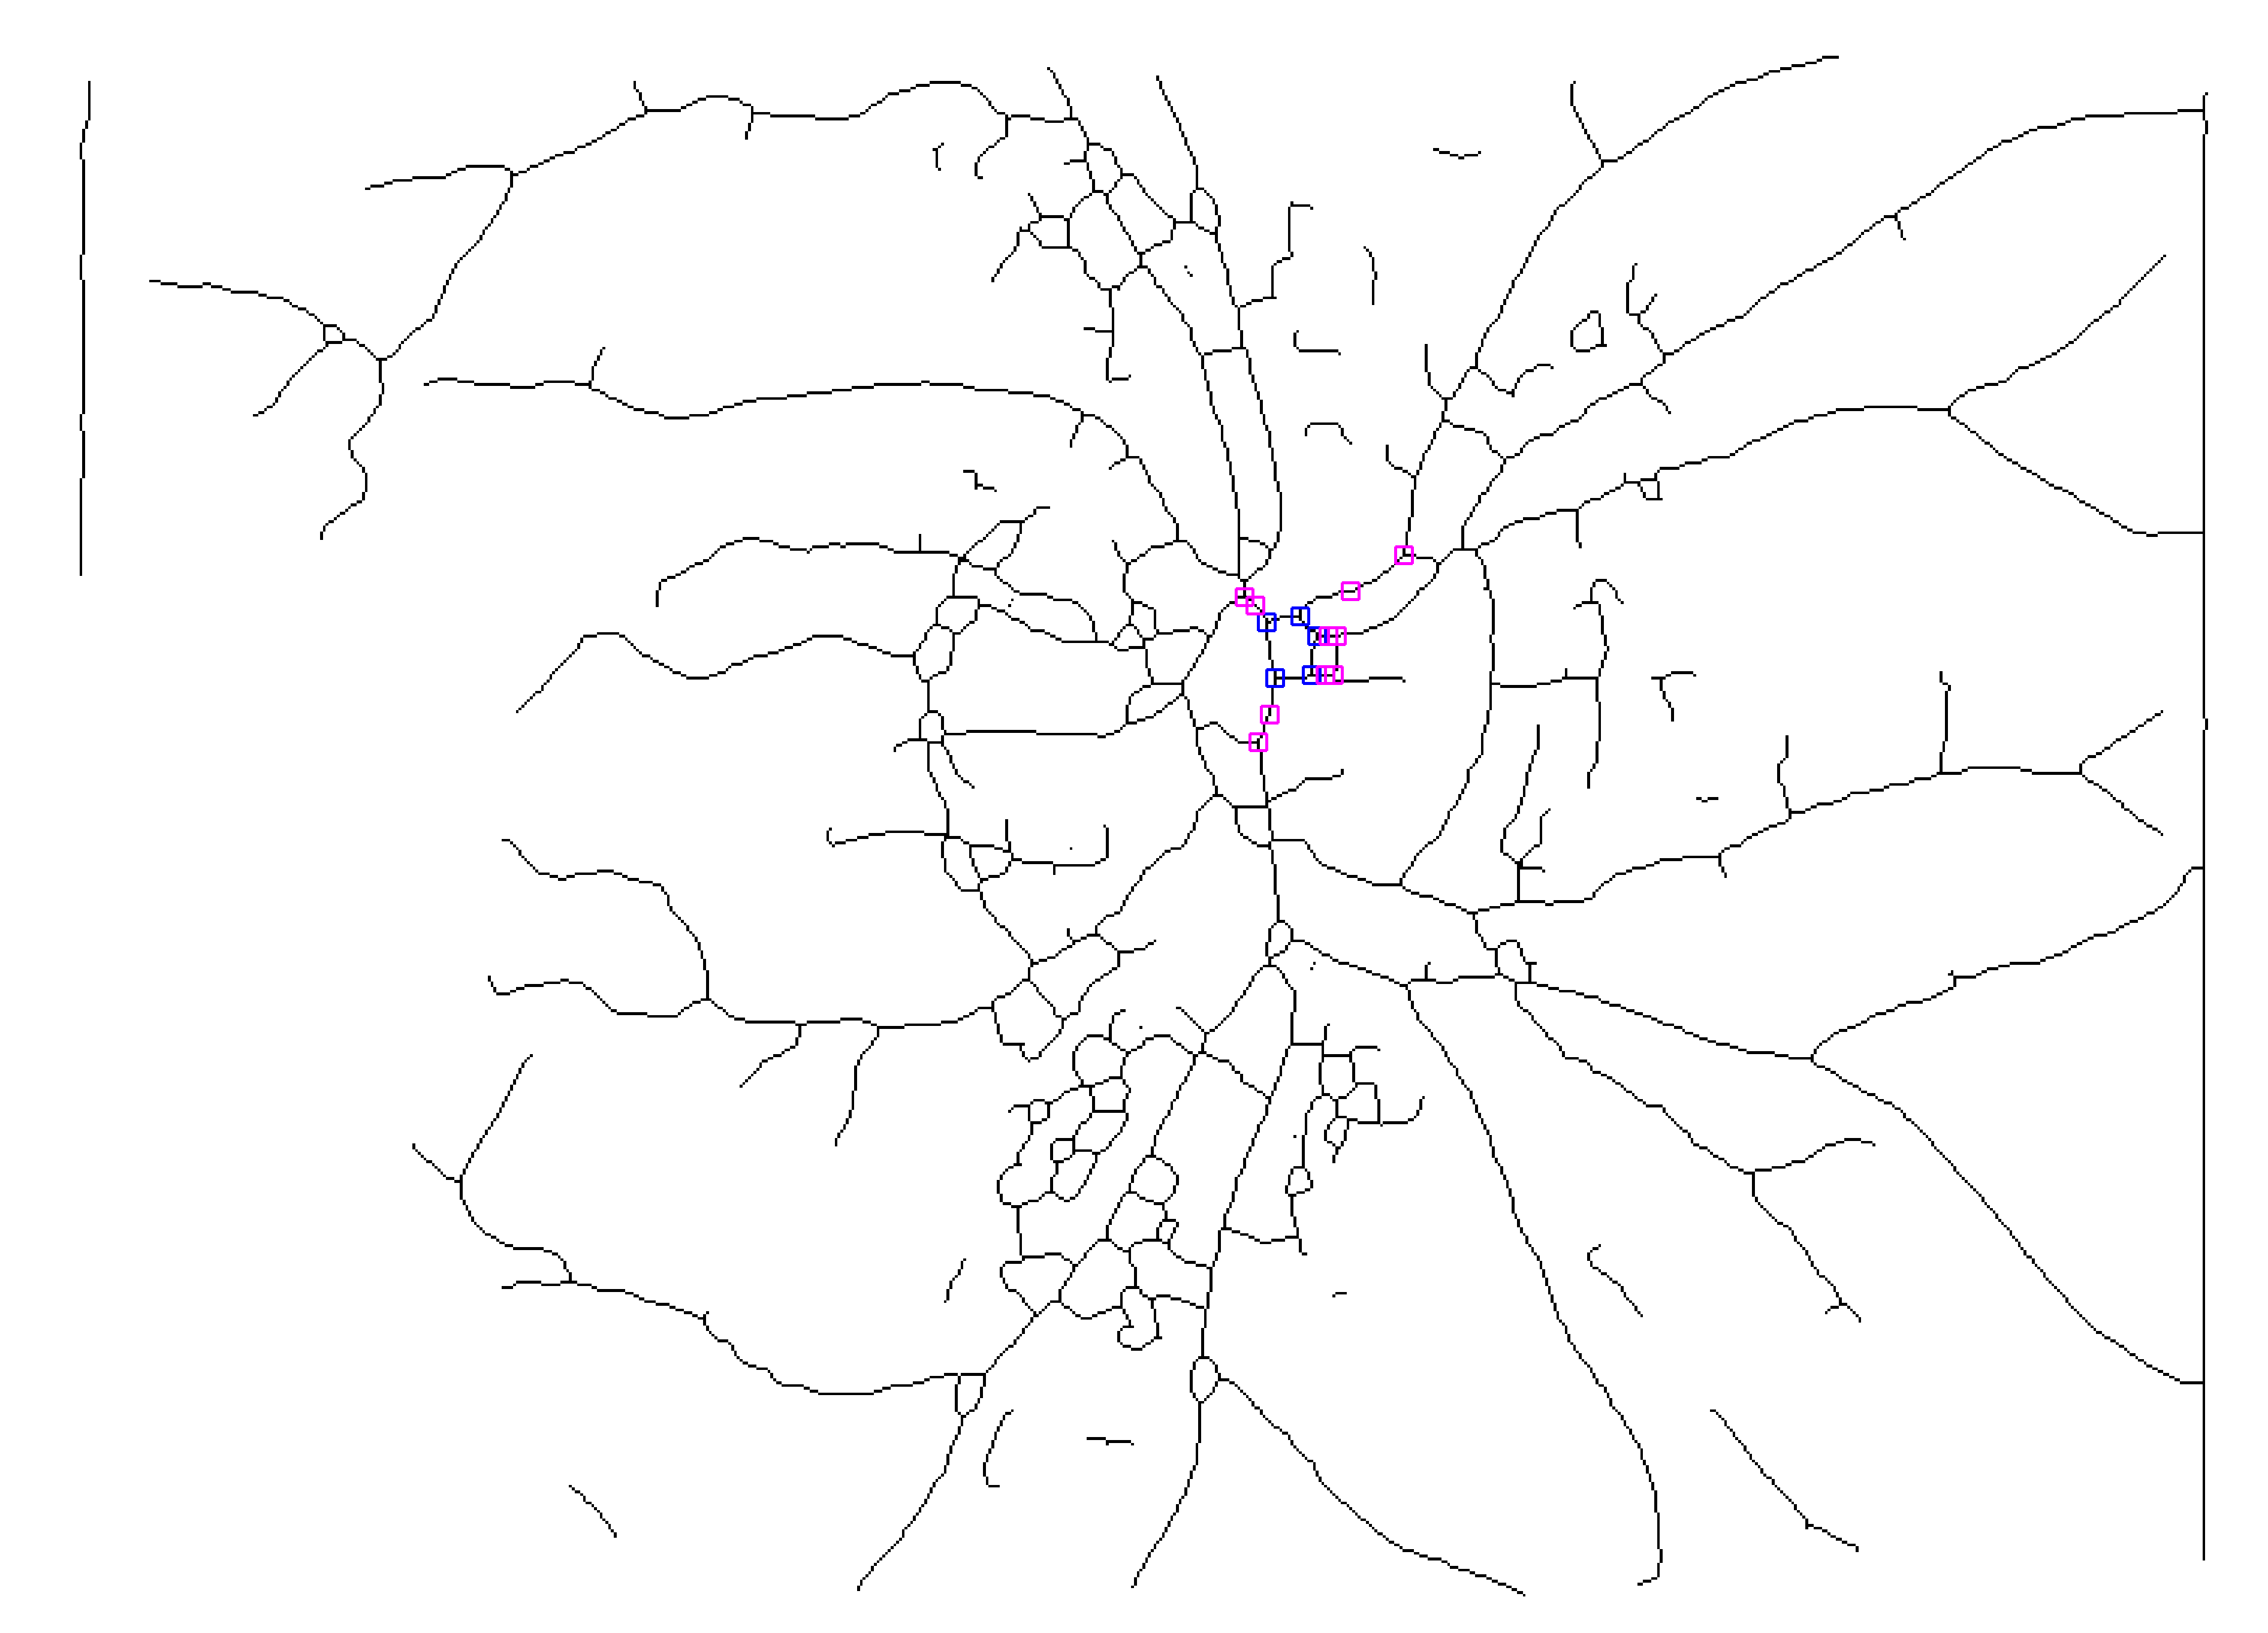
\includegraphics[width=0.6\linewidth]{bw1-cycle-vessel.png}
  \caption{一个五点环-血管结构}
    \label{5bifur-vess}
 \end{figure}
 
关于求解环-血管结构的特征点步骤如下,输入为环结构及连接关系矩阵:
\begin{enumerate}
\item 根据环结构特征点的连接关系矩阵,首先判断参考图像与待配准图像中与环特征点相连的血管末端是否都存在分叉点(或交叉点),并记录两幅图像血管末端均存在分叉点(或交叉点)的特征点的序号。
\item 对血管末端均存在分叉点(或交叉点)的特征点,判断它们的分叉点(或交叉点)是否对应。这主要由分叉点(或交叉点)的分叉角度判断,若角度的平均误差(分叉点为三个角度,交叉点为四个角度)小于阈值,则认为这两个分叉点(或交叉点是)对应的。对于有对应分叉点(或交叉点)的环,其对应分叉点(或交叉点)即为所求的血管末端点。
\item 对血管末端均有分叉点(或交叉点)但不对应、不同时存在分叉点(或交叉点)或分叉点(或交叉点)均不存在的情况,先求解两幅图像的环结构对应边的血管长度并相除确定两幅图像的缩放参数,在两幅图像中与环结构特征点相连的外接血管上截取对应长度血管,从而确定血管末端的坐标。
\item 求解与环结构特征点相连的外接血管中点的血管坐标。
\end{enumerate}
  求解血管长度对于血管中心及末端的点的求解来说是必要的步骤。由于我们采用的视网膜图像为单像素骨架化图像,求解两个环特征点之间的血管长度,相当于进行像素计数。算法步骤如下,其中输入为分叉点(或交叉点)的连接关系矩阵(包含所有与该分叉点相连的分叉点、分支信息),外接目标序号(序号为1 则表明该分叉点(或交叉点)有分支但末端没有分叉点,序号为其他则表示该分叉点存在外接分叉点,该序号即为分叉点(或交叉点));输出为血管的长度,血管的所有像素序号:
\begin{enumerate}
\item 以分叉点(或交叉点)为中心,求其八邻域内像素值为1 的点,该像素个数代表了该分叉点可能的分支数,也决定了下一步血管搜索路径的起始点。
\item 对每一条分支,从起始点(将该起始点加入到stackmap 中备用)开始,求其八邻域内像素值为1 的点,然后判断该点是否属于分叉点(或交叉点)的连接关系矩阵,若是,则该点为分叉点(或交叉点),将该点序号加入到目标向量(targetbifu)中以便后续判断,同时该条分支不再搜寻;不是则将该点加入到stackmap中备用。待该点8 邻域内的点均判断一遍后,以stackmap中的下一个点为起点重复上述步骤,直到stackmap 中所有点都处理完成。
\item 经过以上处理,会将与该分叉点相连的所有分支都搜寻一遍,并将每条分支经过的像素点和血管分支末端的分叉点(若分叉点存在)分别记录在node序列和目标向量中,其中若血管分支末端无分叉点(或交叉点),则该分支的目标向量位置的序号默认为0。但若已知外接目标为分叉点,在算法进行中加入目标向量的某个点等于外接目标分叉点时,便可以中途停止所有分支的寻找,同时计算中node序列中的像素个数得到血管的长度及所有像素序号。若外接目标为没有分叉点的分支,寻找目标向量(targetbifu)中序号为0的点所对应的node序列即为所求分支经过的所有像素点。
\end{enumerate}
一个三分叉点搜索实例如下:
   \begin{figure}[ht!]
   \centering
  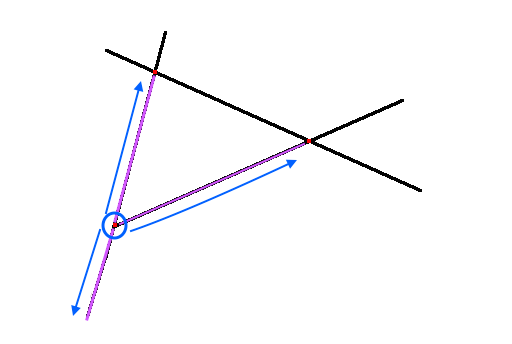
\includegraphics[width=0.5\linewidth]{例子.png}
  \caption{三分叉点搜索实例}
 \end{figure}

其中,针对环上出现的四交叉点情况,需要进一步处理。不同于三分叉点除了环上的两条分支,只有一条外接分支,四交叉点有两条外接分支,这就使得它的外接情况更加复杂:可能存在两个外接分支末端均没有分叉点,两个外接分支末端均存在分叉点及一条外接分支末端存在分叉点,一条外接分支末端没有分叉点的情况。而如果是两个匹配的四交叉点求解环-血管特征点,则可能出现更多情况,但在我们实际处理中,除了对于两个外接分支均不存在分叉点的情况需要进一步处理,其他与上述处理过程均一致。

对于外接目标的两个分支均没有分叉点的情况,由于都是求目标向量中序号为 0 的点,无法确保两幅图像中的两条分支一一对应,因此需要进一步判断:首先确定与该分叉点相连的环上的两个相邻分叉点,选定其中一个相邻分叉点与连个外接分叉点连线,分别计算两个分支与该连线间的角度,根据角度大小调整位置,使两个外接分叉点按一定的顺序排序,如下图~\ref{4bifur}所示。
   \begin{figure}[ht!]
   \centering
  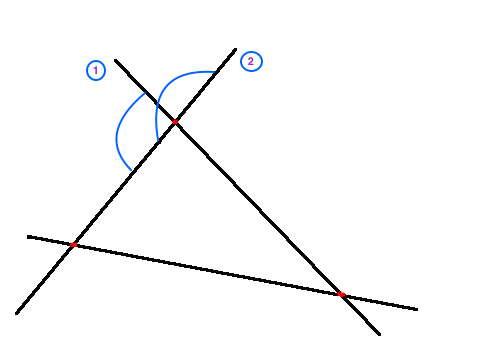
\includegraphics[width=0.5\linewidth]{四分叉.png}
  \caption{两个外接分支均无分叉点的情况}
  \label{4bifur}
 \end{figure}
通过以上步骤,我们获得了匹配的环-血管特征点。

\subsection{相似性变换}
确立了匹配的特征点,接下来是根据特征点选择变换方法,得到图像空间坐标变换参数。几何变换模型的选择对于配准算法的成功至关重要,同时严重依赖于用于配准的数据。通常,几何变换分为刚体与非刚体变换。刚体变换是最简单的变换,由平移和旋转组成。非刚体变换包括相似性变换(由平移,旋转,统一性尺度组成),仿射变换(由平移,旋转,尺度和错切组成),投影变换等。其中平移,旋转,缩放,错切等是常见的图像几何变换方式。 

在欧氏几何里,平移指的是沿着一个给定的方向将一幅图或空间的每个点移动等长的距离。平移变换是一种刚体变换,变换不改变图形的大小、形状和方向,只是位置发生改变。设$(x,y)$为原图像上一点,在水平、垂直方向分别移动$tx$和$ty$,平移后坐标为$(x^{'},y^{'})$,其变换矩阵的齐次坐标表示法为:
\begin{align}
\left[ \begin{array}{c}
x^{'} \\
y^{'}\\
1   
\end{array} \right]
=
\left[ \begin{array}{ccc}
1 & 0 & t\\
0 & 1 & t \\
0 & 0 & 1
\end{array} \right]
\left[ \begin{array}{c}
x\\
y \\
1
\end{array} \right]
\end{align}

   \begin{figure}[ht!]
   \centering
  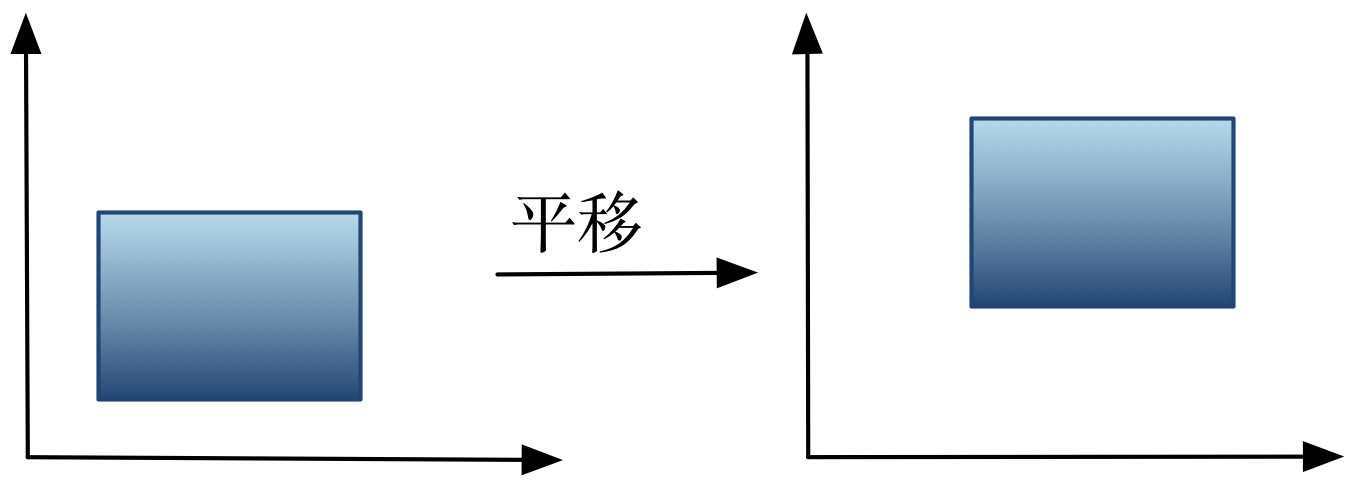
\includegraphics[width=0.7\linewidth]{translation.png}
  \caption{平移示例}
 \end{figure}

在欧氏平面上,平面上的所有点通过绕一固定点转动某个角度$\theta$,变成新的一批点所产生的变换称为旋转变换,旋转前、后的图形全等。设$(x,y)$为原图像上一点,经过旋转变换$\theta$角度后,坐标为$(x^{'},y^{'})$,其变换的矩阵表示形式为:
\begin{align}
\left[ \begin{array}{c}
x^{'} \\
y^{'}\\
1   
\end{array} \right]
=
\left[ \begin{array}{ccc}
cos\theta & -sin\theta & 0 \\
sin\theta & cos\theta & 0 \\
0 & 0 & 1
\end{array} \right]
\left[ \begin{array}{c}
x\\
y \\
1
\end{array} \right]
\end{align}

   \begin{figure}[ht!]
   \centering
  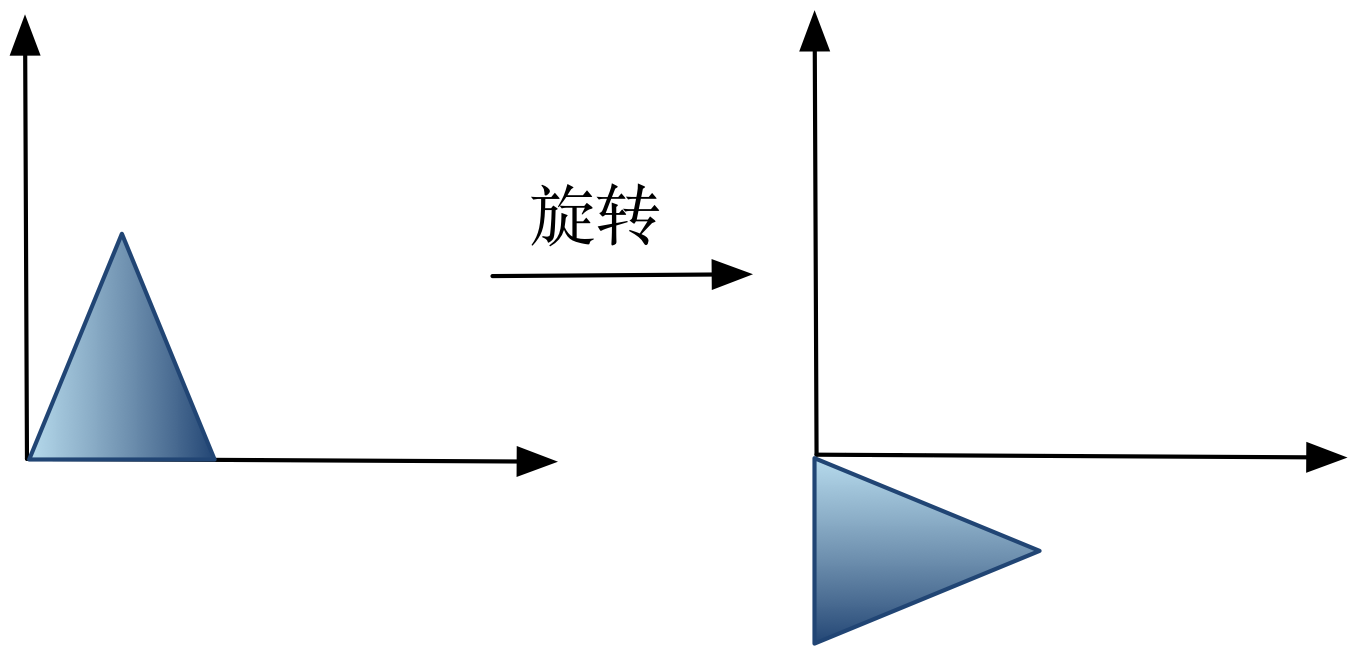
\includegraphics[width=0.7\linewidth]{rotation.png}
  \caption{旋转示例}
 \end{figure}
 
 在欧氏几何中,缩放是指按固定的缩放因子在所有方向扩大或缩小一个物体。设$(x,y)$为原图像上一点,缩放后坐标为$(x^{'},y^{'})$,$sx$为水平方向的缩放因子,$sy$为垂直方向的缩放因子,其变换的矩阵表示形式为:
 \begin{align}
\left[ \begin{array}{c}
x^{'} \\
y^{'}\\
1   
\end{array} \right]
=
\left[ \begin{array}{ccc}
sx & 0 & 0 \\
0 & sy & 0 \\
0 & 0 & 1
\end{array} \right]
\left[ \begin{array}{c}
x \\
y\\
1
\end{array} \right]
\end{align}

   \begin{figure}[ht!]
   \centering
  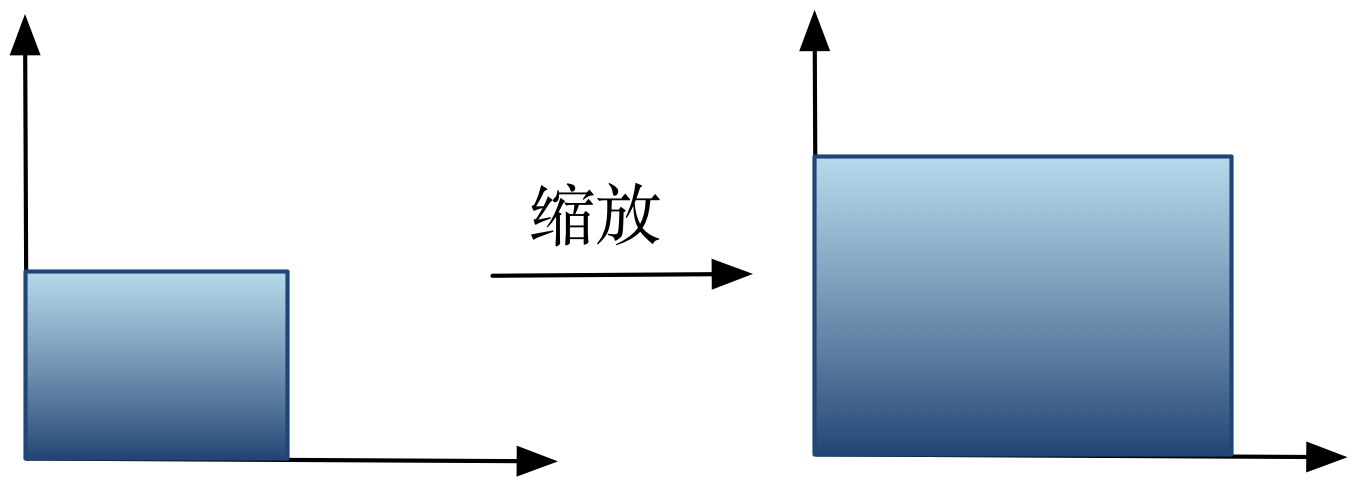
\includegraphics[width=0.7\linewidth]{scale.png}
  \caption{缩放示例}
 \end{figure}
 
 错切变换又称剪切变换,指的是保持图形上各点的某一坐标值不变,而另一坐标值关于该坐标值呈线性变换,类似于四边形、方形变平行四边形,任意一边都可以被拉长的过程。错切分为两种情况:水平方向错切和垂直方向错切,设$(x,y)$为原图像上一点,错切后坐标为$(x^{'},y^{'})$,变换的矩阵表示形式如下。
 \begin{align}
\left[ \begin{array}{c}
x^{'} \\
y^{'}
\end{array} \right]
=
\left[ \begin{array}{ccc}
1 & \tan \alpha \\
0 & 1
\end{array} \right]
\left[ \begin{array}{c}
x \\
y
\end{array} \right]
\label{shuiping}
\end{align}

  \begin{align}
\left[ \begin{array}{c}
x^{'} \\
y^{'}
\end{array} \right]
=
\left[ \begin{array}{ccc}
1 & 0 \\
\tan \alpha & 1
\end{array} \right]
\left[ \begin{array}{c}
x \\
y
\end{array} \right]
\label{chuizhi}
\end{align}
    \begin{figure}[ht!]
   \centering
  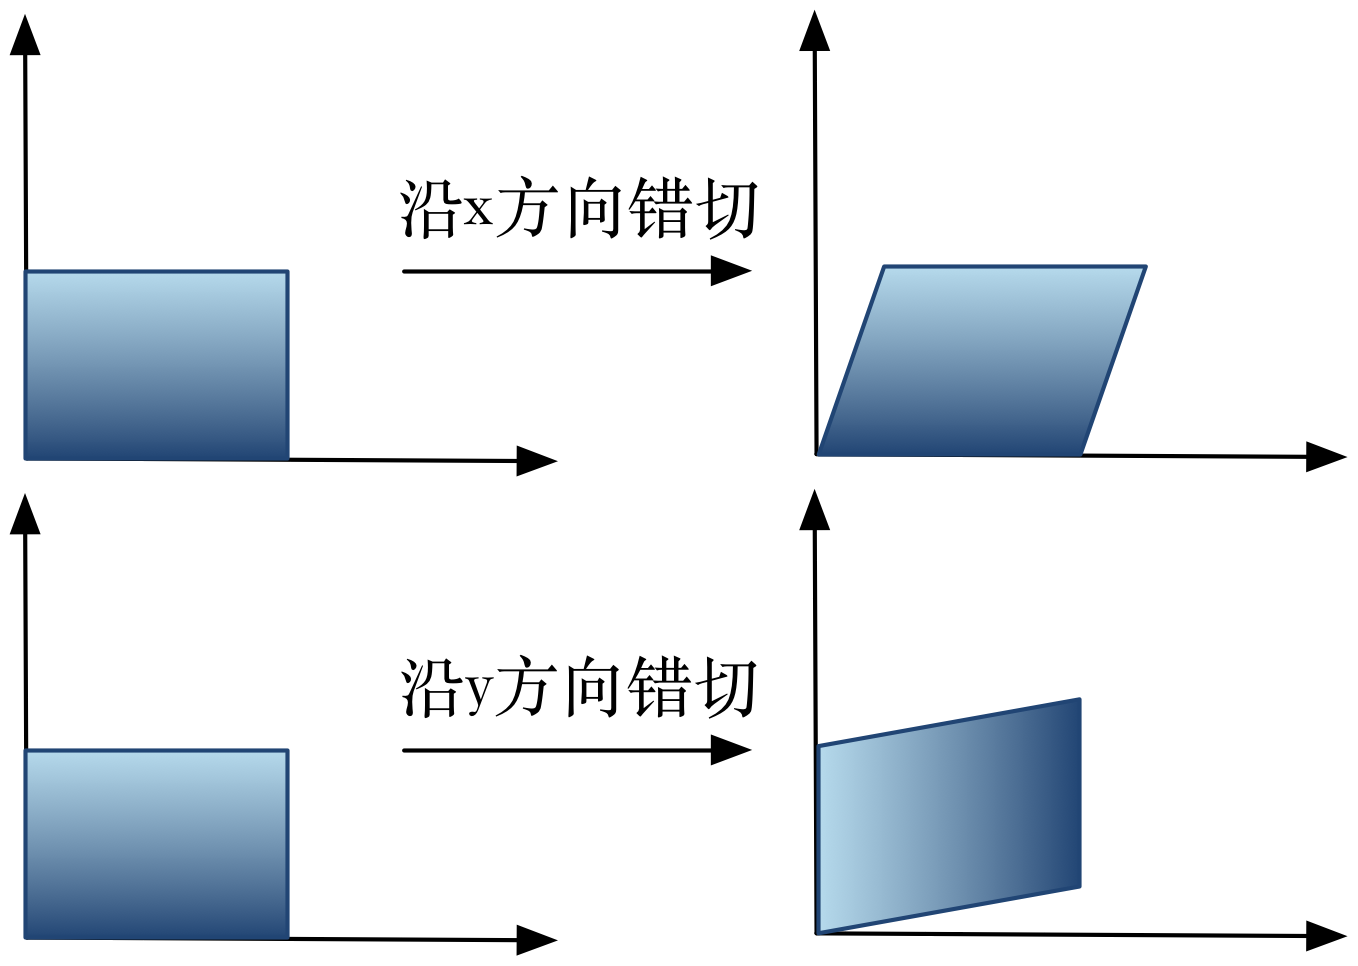
\includegraphics[width=0.7\linewidth]{shear.png}
  \caption{错切示例}
 \end{figure}

公式~\ref{shuiping}为水平方向错切,公式~\ref{chuizhi}为垂直方向错切。设$shx$为水平方向的错切因子,$shy$为垂直方向的错切因子,一个水平方向和垂直方向错切的复合变换的矩阵表示形式为:
 \begin{align}
\left[ \begin{array}{c}
x^{'} \\
y^{'}\\
1   
\end{array} \right]
=
\left[ \begin{array}{ccc}
1 & shx & 0 \\
shy & 1& 0 \\
0 & 0 & 1
\end{array} \right]
\left[ \begin{array}{c}
x \\
y\\
1
\end{array} \right]
\end{align}
	 	
仿射变换是多种图像配准方法中常用的变换模型,是一种二维坐标到二维坐标之间的线性变换。它有两个特点:直线经过变换之后依然是直线,圆弧变化后还是圆弧 ,这个特点被称为“平直性”;平行线经过变换后还是平行线,直线上点的位置顺序不变,但向量间的夹角可能会发生变化,这个特点称作“平行性”~\cite{liuwei}。仿射变换可以经过坐标系的平移,旋转,缩放,翻转和错切的复合变换得到。仿射变换可以被定义为:
\begin{equation}
\begin{split}		
X=ax+by+c\\
Y=dx+ey+f		
\end{split}
\end{equation}		
 \begin{align}
\left[ \begin{array}{c}
X \\
Y \\
1   
\end{array} \right]
=
\left[ \begin{array}{ccc}
a & b & c \\
d & e & f \\
0 & 0 & 1
\end{array} \right]
\left[ \begin{array}{c}
x \\
y\\
1
\end{array} \right]
\end{align}

其中,$a$、$b$、$c$、$d$、$e$和$f$参数代表平移,旋转,缩放,翻转和错切等参数的复合,仿射变换至少需要三对非共线的匹配特征点以决定变换的这六个参数。
与仿射变换不同的是,相似性变换可以看作是由平移,旋转,缩放及翻转组成的,变换后其角度不会发生变化,定义如下:
\begin{equation}
\begin{split}		
X=xs\cos\phi-ys\sin\phi+a\\
Y=xs\sin\phi+ys\cos\phi+b	
\end{split}
\end{equation}
 \begin{align}
\left[ \begin{array}{c}
X \\
Y \\
1   
\end{array} \right]
=
\left[ \begin{array}{ccc}
1 & 0 & a\\
0 & 1 & b \\
0 & 0 & 1
\end{array} \right]
\left[ \begin{array}{ccc}
cos\theta & -sin\theta & 0 \\
sin\theta & cos\theta & 0 \\
0 & 0 & 1
\end{array} \right]
\left[ \begin{array}{ccc}
s & 0 & 0\\
0 & s & 0 \\
0 & 0 & 1
\end{array} \right]
\left[ \begin{array}{c}
x \\
y\\
1
\end{array} \right]
\end{align}

其中$s$代表尺度,$\phi$代表旋转角度,$(a,b)$代表了参考图像与待配准图像间的平移距离,相似性变换至少需要两对匹配的特征点来求得上述的参数。

很明显,我们提出的环-血管结构对于平移、旋转和缩放是不变的,但因为特征点角度及分支间角度的存在,对于错切是可变的,因此本文中选择相似性变换作为配准的变换模型。在后续的实验对比中,我们对仿射性变换、相似性变换及多项式变换进行了对比,验证了选择相似性变换的优越性。

根据我们提供的多对特征点输入坐标值,通过最小二乘法等方法求解变换模型,可得变换的参数,然后对待配准图像进行相应变换,可得最终的配准结果,这里求得变换参数及进行变换主要采用了MATLAB的\emph{cp2tform}函数和\emph{imtransfrom}函数。为了使配准结果易于观察和对比,我们将参考图像骨架化图像与待配准图像变换后的结果通过图像处理的方法相融合,如图 ~\ref{initial}中所示配准结果为运用环-血管特征点的局部初始配准结果。
\begin{figure}[ht!]
  \centering
  \begin{minipage}[b]{0.45\linewidth} 
  \centering
  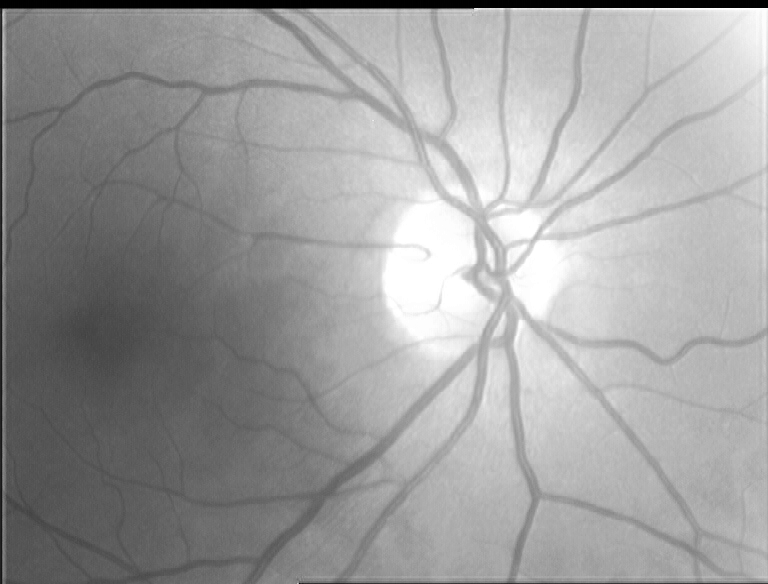
\includegraphics[width=0.9\linewidth]{R128.png}
  \centerline{(a) 参考图像}\medskip
    \end{minipage}
\begin{minipage}[b]{0.45\linewidth}
  \centering
  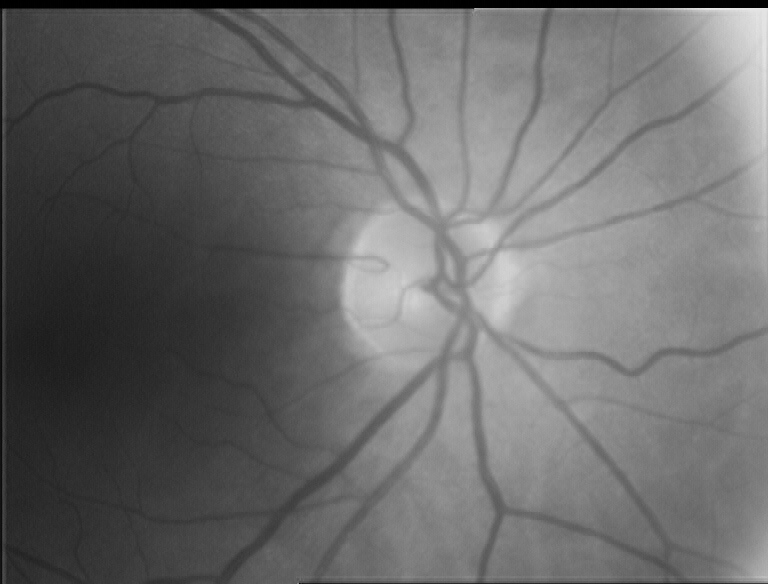
\includegraphics[width=0.9\linewidth]{R225.png}
 \centerline{(b) 待配准图像}\medskip
   \end{minipage}  
  \begin{minipage}[b]{0.45\linewidth}
    \centering
  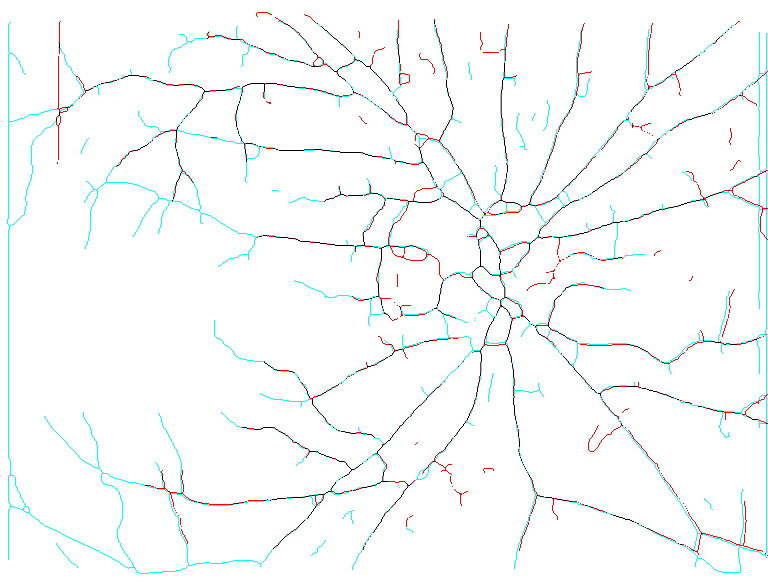
\includegraphics[width=0.9\linewidth]{128-225-initial-reg.png}
 \centerline{(c) 骨架化图像配准结果}\medskip
   \end{minipage}  
  \begin{minipage}[b]{0.45\linewidth}
    \centering
  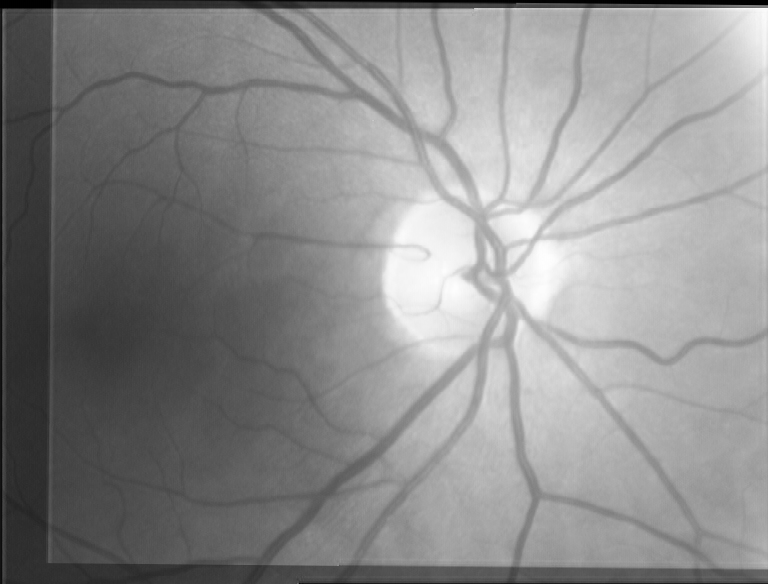
\includegraphics[width=0.9\linewidth]{128-225-initial-result.png}
   \centerline{(d) 原始图像配准结果}\medskip
   \end{minipage}  
  \caption{一对视网膜图像初次配准结果示例}
    \label{initial}
 \end{figure}

\section{全局最终配准}
\subsection{全局配准原理}
我们从局部初始配准的结果可以看出,一部分视网膜图像取得了较好的配准结果,而一部分配准结果存在如下问题:在离环结构较近的区域配准比较准确,参考图像与待配准图像的重合度较高,而在离环结构较远的区域,尤其是图像的边缘部分,经常会出现分支整体偏差的情况(如图 ~\ref{unalign}中所示,左边的一条分叉点分支有较大偏离),而且如果环结构位置较偏僻,可能分支偏差情况更加明显。
 \begin{figure}[ht!]
  \centering
  \begin{minipage}[b]{0.45\linewidth} 
      \centering 
  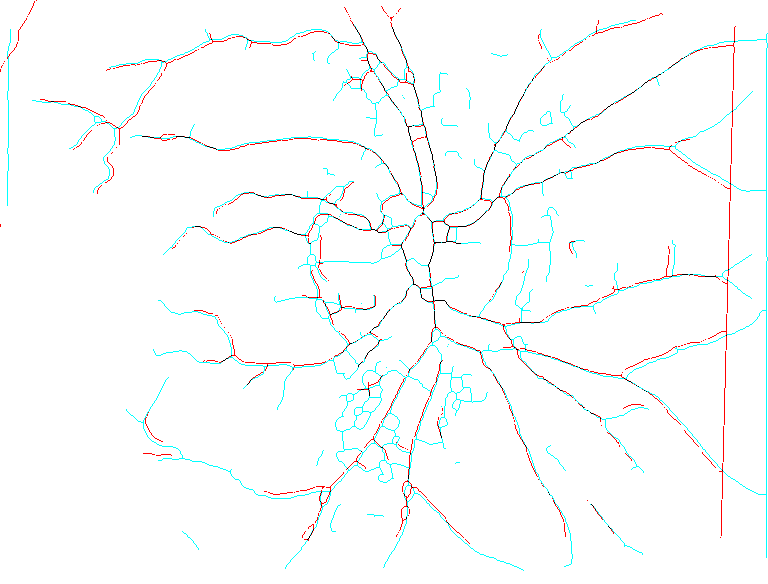
\includegraphics[width=0.9\linewidth]{067-119-initial_reg.png}
        \centerline{(a)}\medskip
    \end{minipage}
  \begin{minipage}[b]{0.45\linewidth} 
      \centering 
  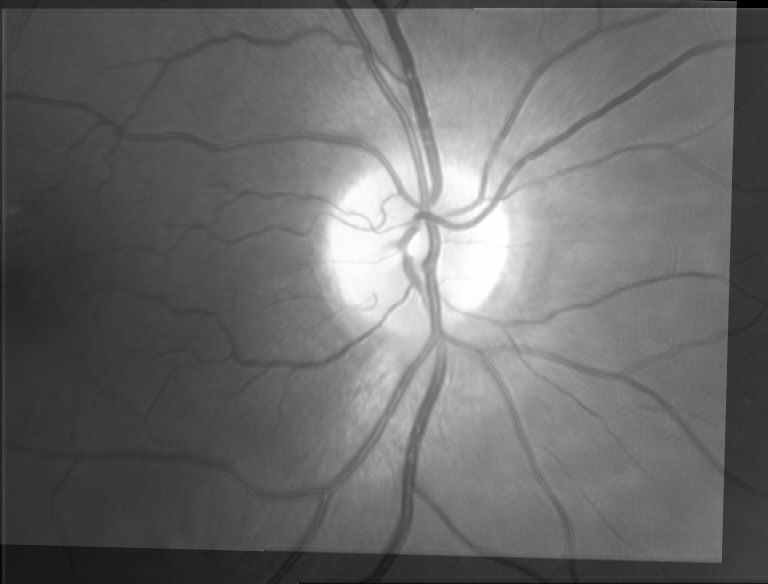
\includegraphics[width=0.9\linewidth]{067-119-initial_result.png}
    \centerline{(b)}\medskip
      \end{minipage}
  \caption{分支血管未对齐的局部初始配准结果}
    \label{unalign}
 \end{figure}

经过分析,我们得出结论,环-血管特征点虽然可以满足配准的准确性要求,但仍缺乏足够的鲁棒性,因为这些点仅仅可以覆盖那些拥有复杂血管网络,易构成环结构的局部区域,而对于远离这些环结构区域的局部区域来说,易出现分支血管未对齐的情况。同时我们观察了这些远离环结构区域的特点,可以看出,这些局部区域虽然可能不存在环结构,但是由于分叉点(或交叉点)广泛分布的特性,它们多半存在着分叉点(或交叉点),如果我们将这些因为分支血管未对齐而导致不能正确对应的分叉点(或交叉点)找到并保证它们能够正确配准,那么该分叉点(或交叉点)所在的血管分支也会相应对齐,从而修正初始局部配准造成的部分局部未对齐情况的发生。

考虑到以上情况,我们提出了将配准从局部扩展到全局,由局部初始配准的结果找到未对齐的血管分叉点(或交叉点),构成环-血管-分叉点特征点集合,进行再次配准的改进。

\subsection{全局配准过程}
首先,我们要找到全局区域内未对齐的分叉点(或交叉点),这部分的过程如下:以参考图像的一个分叉点(或交叉点)为中心,取其$11\times11$像素大小的邻域,寻找待配准图像变换后的图像在此邻域内的所有分叉点(或交叉点)。若不存在分叉点(或交叉点),则不进行操作。若此邻域内存在分叉点(或交叉点),则计算所有分叉点(或交叉点)的分支角度,并得出与参考图像的目标分叉点(或交叉点)的各个分支角度相比的平均误差。在所有分叉点(或交叉点)里选择平均误差最小的一个点,查看其误差是否小于给定阈值,若是则认为该分叉点(或交叉点)与参考图像中的分叉点(或交叉点)是对应分叉点(或交叉点)。然后分别计算该对应分叉点(或交叉点)在图像中的行数与列数,并求得横纵坐标,从而求得两者之间的像素距离,如公式~\ref{pixel-dis}所示:
\begin{equation}
\begin{split}
D(i)&=\sqrt{(dx^2+dy^2)}\\
dx&=bw1_x(i)-outbw2_x(i)\\
dy&=bw1_y(i)-outbw2_y(i)
\end{split}
\label{pixel-dis}
\end{equation}

其中$bw1$代表参考图像,$bw2$代表待配准图像,$outbw2$代表$bw2$配准后的变换图像。

如果求得的分叉点的像素距离大于阈值3,则认为该对应分叉点未对齐,我们将此对未对齐分叉点加入到临时分叉点(或交叉点)点集当中,以供后续处理。这个阈值是由实验得出的经验值,然后我们根据这个步骤将所有分叉点搜索一遍。

找到所有未对齐的分叉点(或交叉点)后,需要解决的另一个问题是由变换后的待配准图像的分叉点(或交叉点)找到其变换前,即原始图像的对应分叉点(或交叉点),这样才能得到正确的未对齐分叉点(或交叉点)点集。其解决方法是:通过MATLAB的\emph{tformfwd}函数及待配准图像的变换矩阵,将待配准图像中的每个分叉点(或交叉点)进行二维空间变换,得到变换后的分叉点(或交叉点),得到两者之间的对应关系。再通过与临时分叉点(或交叉点)点集中的待配准图像变换后的点进行比对,从而找到对应变换前的分叉点(或交叉点)。

通过以上步骤,我们得到了全局范围内未对齐的分叉点(或交叉点)点集,将该点集与环-血管点集结合,得到了最终的环-血管-分叉点特征点集。然后,与局部初始变换一样,我们采用相似性变换对环-血管-分叉点特征点集进行处理,得到变换参数,再由该参数完成图像的变换,最终得到了全局二次配准的结果。图 ~\ref{align}为与图~\ref{unalign}对应的骨架化及原始图像全局二次配准结果,由观察可知,该视网膜图像配准结果左右两边的血管未对齐的情况得到了有效修正,整体配准效果也有了较大的改善,参考图像与待配准图像的骨架结果重合率较高。
 \begin{figure}[ht!]
  \centering
  \begin{minipage}[b]{0.48\linewidth} 
      \centering 
  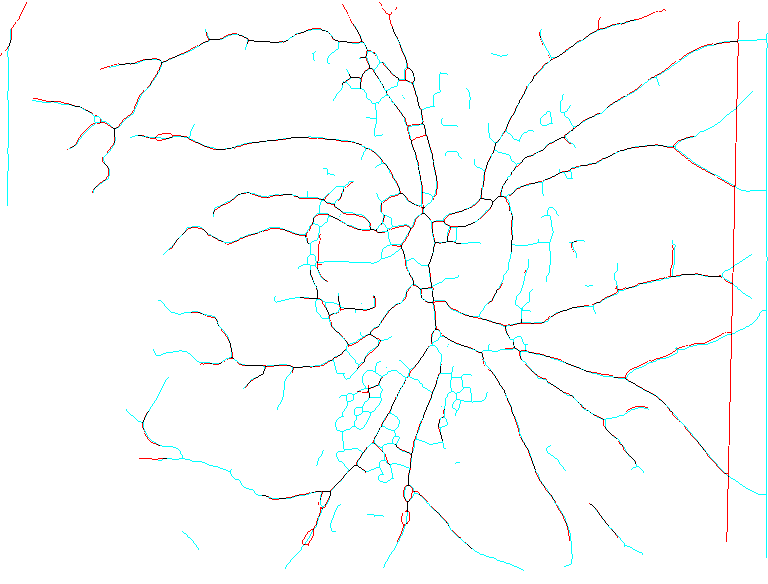
\includegraphics[width=0.9\linewidth]{067-119-local_reg.png}
        \centerline{(a)}\medskip
    \end{minipage}
  \begin{minipage}[b]{0.48\linewidth} 
      \centering 
  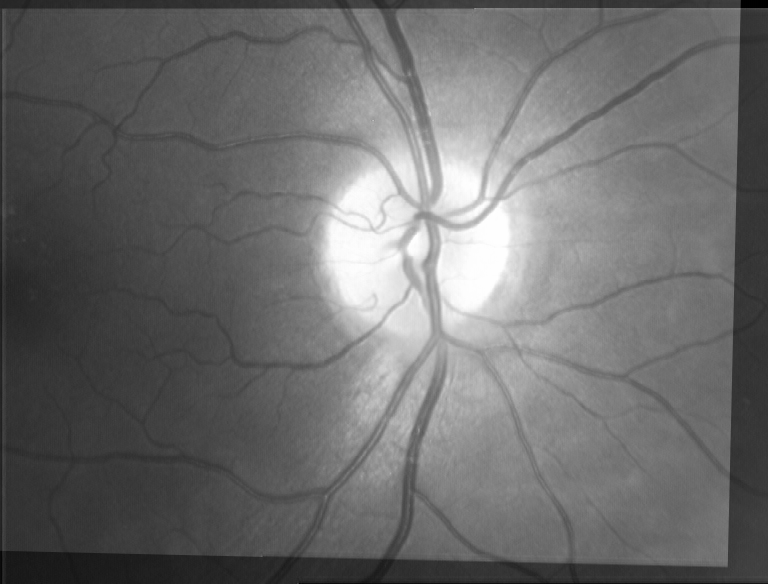
\includegraphics[width=0.9\linewidth]{067-119-result.png}
    \centerline{(b)}\medskip
      \end{minipage}
  \caption{与图~\ref{unalign}对应的全局最终配准结果}
    \label{align}
 \end{figure}
 
 纵观配准的整个流程,我们使用了环结构,环-血管结构,环-血管-分叉点三级特征用来进行配准。总体来说,使用环-血管-分叉点特征的最终配准取得最优的配准结果。然而,我们观察发现在某些情况下,加上血管特征点,或者最终的全局分叉点,反而会使配准结果变差。有时在一组配准图像中,简单的环结构即可取得较理想的配准结果。因此我们提出了对从局部到全局配准策略的一种改进:分别计算环结构,环-血管结构,环-血管-分叉点下的所有配准结果,然后根据下章介绍的误差度量方法选择出最优的配准结果。关于我们的二级配准方法与三种特征选择方法进行的实验对比结果可在第五章对比实验中看到。
 
 \section{本章小结}
 本章描述了从局部到全局的配准策略。在构造的多环结构基础上,我们对简单的环结构进行了扩展,通过求解与环结构相连的分叉点(或交叉点),及两者之间的血管的中点,构造了环-血管结构,作为变换的输入。重点介绍了多种图像几何变换模型,考虑到提出的环结构的特点,最终选择相似性变换作为变换的模型,由此求得图像空间坐标变换参数,最后由坐标变换参数进行了局部的初次配准。经过局部的初次配准后,由实验结果分析可得:在远离环结构区域的部分区域会出现血管分支未对齐的情况,而在这些区域虽然不一定有环结构存在,但普遍存在分叉点,如果我们将未对齐的分叉点对齐,该分叉点所在的血管分支也会相应对齐。由此,我们提出了环-血管-分叉点的特征点结构,将确认过的未对齐的分叉点加入到特征点集,进行了第二次的全局配准。经过从局部到全局的配准,最大限度的提高了配准的准确度,实验结果表明我们的从局部到全局的配准具有较好的效果。     
 
